\newSection{Experiments}

\subsection{Overview}

%-----------------------------------------------
% Overview of Experimental Objectives
%-----------------------------------------------
\begin{frame}[t]{Experimental Objectives}
    \textbf{Goal:} Validate that \emph{HairStep} reduces the domain gap between synthetic and real data, thereby improving single-view 3D hair modeling quality.

    \vspace{5pt}
    \textbf{Key Objectives to Validate:}
    \begin{itemize}
        \item Demonstrate that \emph{HairStep} outperforms traditional orientation-based methods.
        \item Show improved 3D hair reconstruction on synthetic and real images.
        \item Introduce and validate new metrics (\emph{HairSale} and \emph{HairRida}) for objective evaluation.
    \end{itemize}
\end{frame}

%-----------------------------------------------
% Experimental Setup
%-----------------------------------------------
\begin{frame}[t]{Overview of Core Experiments}
    \begin{enumerate}
        \item \textbf{HairStep Extraction}
        \begin{itemize}
            \item Compare \emph{HairStep}'s strand maps with orientation maps generated using Gabor filters.
            \item Evaluate depth maps extracted using different strategies within the \emph{HairStep} framework.
        \end{itemize}

        \item \textbf{Single-View 3D Hair Modeling}
        \begin{itemize}
            \item Compare the quality of 3D hair reconstruction with existing orientation-based methods.
        \end{itemize}

        \item \textbf{Intermediate Representation Evaluation}
        \begin{itemize}
            \item Assess the impact of different intermediate representations on 3D reconstruction quality.
            \item Evaluate performance on both synthetic and real data using various methods.
        \end{itemize}

        \item \textbf{Ablation Study}
        \begin{itemize}
            \item Experiment with different depth estimation strategies within the \emph{HairStep} framework.
            \item Evaluate their impact on the final 3D hair reconstruction quality.
        \end{itemize}
    \end{enumerate}
\end{frame}

\subsection{Datasets}

%-----------------------------------------------
% Datasets
%-----------------------------------------------
\begin{frame}[t]{Datasets}
    \textbf{Synthetic Dataset:} \emph{USC-HairSalon}~\cite{Hu2015SingleviewHM}
    \begin{itemize}
        \item Contains 343 3D hair models, each with multiple camera views.
    \end{itemize}

    \vspace{5pt}
    \textbf{Real Datasets:} \emph{HiSa} (Strand Map Annotation) and \emph{HiDa} (Depth Annotation)
    \begin{itemize}
        \item \emph{HiSa}: 1,250 real portrait images with dense, pixel-level strand direction annotations.
        \item \emph{HiDa}: 1,250 real portrait images with carefully annotated relative depth pairs.
    \end{itemize}
\end{frame}

\subsection{Evaluation Metrics}

%-----------------------------------------------
% Evaluation Metrics Overview
%-----------------------------------------------
\begin{frame}[t]{Evaluation Metrics}
    \textbf{Quantitative Evaluation:}
    \begin{itemize}
        \item \textbf{For Real Data:}
        \begin{itemize}
            \item \emph{HairSale}: Mean angular error of predicted strand directions.
            \item \emph{HairRida}: Accuracy of predicted relative depth orderings.
        \end{itemize}
        \item \textbf{For Synthetic Data:}
        \begin{itemize}
            \item \emph{Orientation Error}: $L_2$ error between predicted and ground-truth 3D orientation fields.
            \item \emph{Occupancy Accuracy}: Precision of predicted 3D occupancy fields relative to ground truth.
        \end{itemize}
    \end{itemize}

    \vspace{5pt}
    \textbf{Qualitative Evaluation:}
    \begin{itemize}
        \item \emph{Visual Quality}: Subjective assessment of reconstructed geometry.
        \item \emph{User Study}: Preferences gathered from human subjects comparing reconstruction results.
    \end{itemize}
\end{frame}

%-----------------------------------------------
% HairSale Metric
%-----------------------------------------------
\begin{frame}[t]{Evaluation Metric: \emph{HairSale}}
    \emph{HairSale}: Mean Angular Error of Strand Directions.

    \begin{equation*}
        \text{HairSale} = \frac{1}{K} \sum_{i=1}^{K} \arccos\bigl( V(O_r(x_i)) \cdot V(O_{gt}(x_i)) \bigr)
    \end{equation*}

    \begin{itemize}
        \item \textbf{Notation:}
        \begin{itemize}
            \item $K$: Number of pixels within the overlap of predicted and ground-truth masks.
            \item $V(O_r(x_i))$: Unit vector of predicted orientation at pixel $x_i$.
            \item $V(O_{gt}(x_i))$: Unit vector of ground-truth orientation at pixel $x_i$.
        \end{itemize}
    \end{itemize}
\end{frame}

%-----------------------------------------------
% HairRida Metric
%-----------------------------------------------
\begin{frame}[t]{Evaluation Metric: \emph{HairRida}}
    \emph{HairRida}: Relative Depth Ordering Accuracy.

    \begin{equation*}
        \text{HairRida} = \frac{1}{Q} \sum_{i=1}^{Q} \max\bigl(0, r_i \cdot \text{sign}(D_r(p_{i1}) - D_r(p_{i2}))\bigr)
    \end{equation*}

    \begin{itemize}
        \item \textbf{Notation:}
        \begin{itemize}
            \item $Q$: Number of annotated pixel pairs.
            \item $r_i$: Ground-truth relative depth order for pair $i$ ($+1$ or $-1$).
            \item $D_r(p_{i1})$, $D_r(p_{i2})$: Predicted depth values at the corresponding pixels.
        \end{itemize}
    \end{itemize}
\end{frame}

%-----------------------------------------------
% Metrics Visualization
%-----------------------------------------------
\begin{frame}[t]{Evaluation Metrics Illustration}
    \begin{figure}
        \centering
        \includegraphics[width=0.95\textwidth]{assets/figures/eval/metrics/metrics.png}
        \caption{Illustration of the \emph{HairSale} and \emph{HairRida} metrics.}
    \end{figure}
\end{frame}

%-----------------------------------------------
% Qualitative Evaluation Examples
%-----------------------------------------------
\begin{frame}[t]{Qualitative Evaluation Examples}
    \begin{figure}
        \centering
        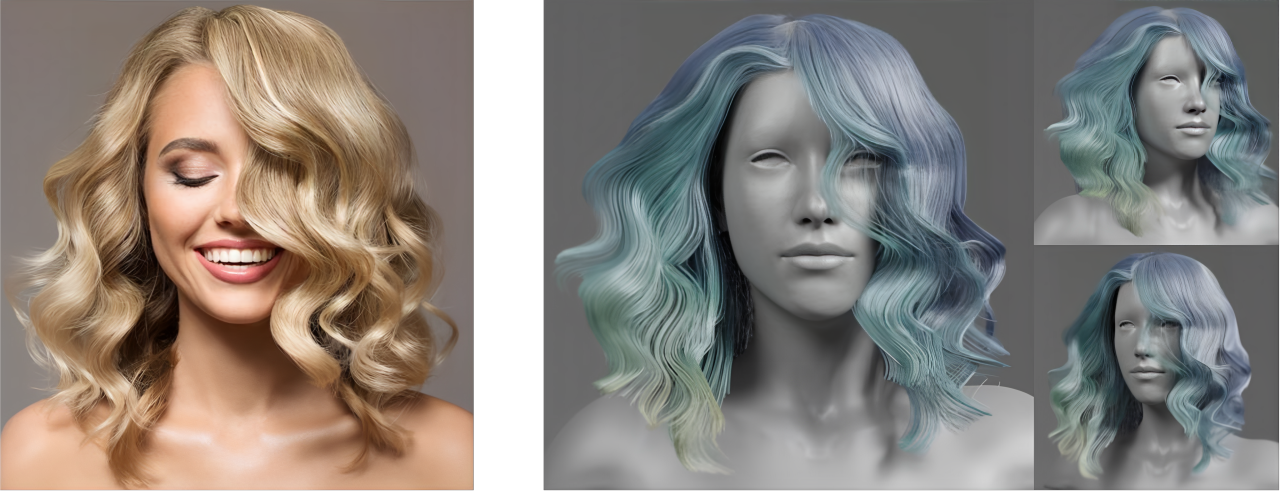
\includegraphics[width=0.9\textwidth]{assets/figures/eval/metrics/input-output.png}
        \caption{Comparing input images with reconstructed 3D hair models.}
    \end{figure}
\end{frame}

\subsection{HairStep Extraction Evaluation}

%-----------------------------------------------
% HairStep Extraction Introduction
%-----------------------------------------------
\begin{frame}[t]{HairStep Extraction Evaluation}
    \textbf{Objective:} Evaluate the quality of strand and depth maps extracted using \emph{HairStep}.

    \vspace{5pt}
    \begin{itemize}
        \item \textbf{Strand Maps:}
        \begin{itemize}
            \item Compare \emph{HairStep}'s strand maps with orientation maps generated using Gabor filters.
            \item Quantitative evaluation using the \emph{HairSale} metric (undirected).
        \end{itemize}
        \item \textbf{Depth Maps:}
        \begin{itemize}
            \item Compare the impact of different depth estimation strategies within the \emph{HairStep} framework.
            \item Quantitative evaluation using the \emph{HairRida} and $L_1$ loss metrics.
        \end{itemize}
    \end{itemize}
\end{frame}

\subsubsection{Strand Map Extraction}

%-----------------------------------------------
% Strand Maps Qualitative Comparison
%-----------------------------------------------
\begin{frame}{Strand Map Extraction: Qualitative Comparison}
    \begin{figure}
        \centering
        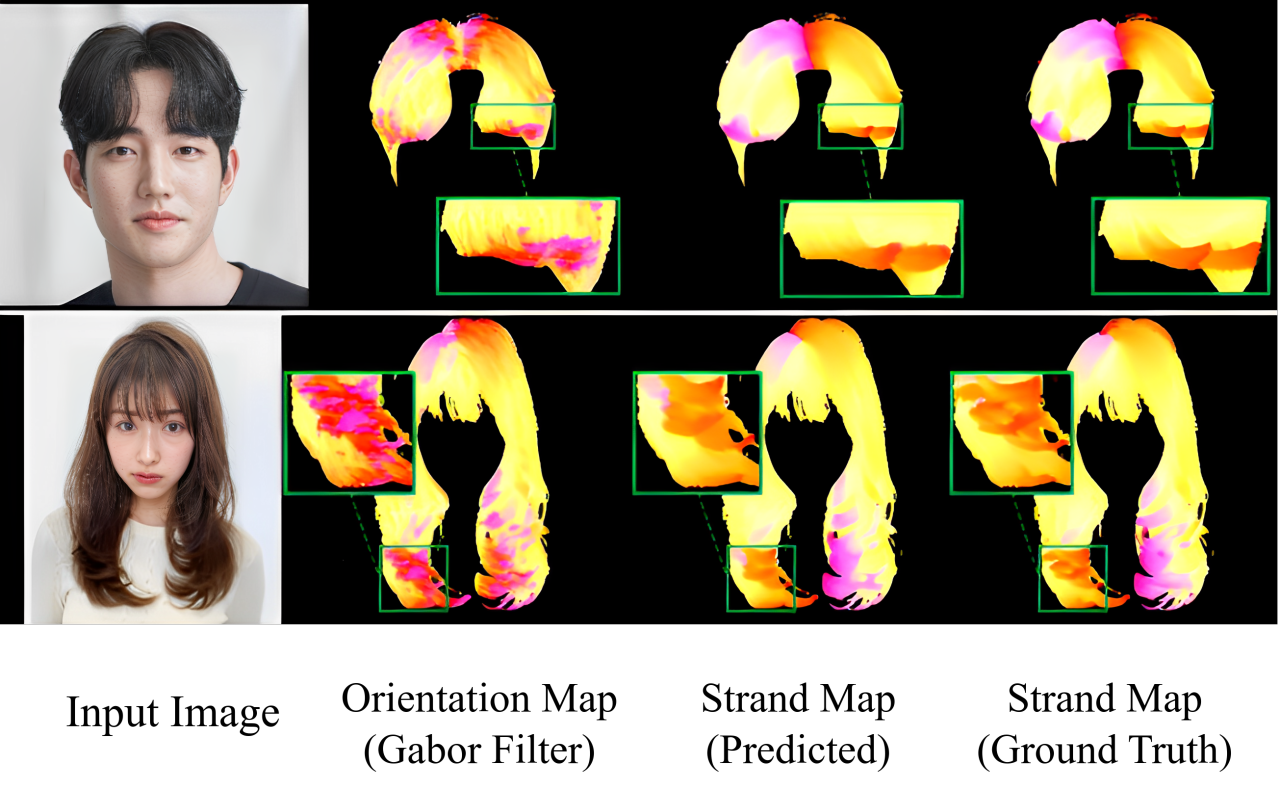
\includegraphics[width=0.65\textwidth]{assets/figures/eval/hairsale/strand-prediction-comparison.png}
        \caption{Qualitative comparison of predicted strand maps versus ground truth.}
    \end{figure}
\end{frame}

%-----------------------------------------------
% Strand Maps Quantitative Comparison
%-----------------------------------------------
\begin{frame}[t]{Strand Map Extraction: Quantitative Results}
    Using the \emph{HairSale} metric for evaluation, \emph{HairStep}'s strand map is converted to an undirected form to match Gabor filters' orientation ambiguity.

    \vspace{5pt}
    \begin{table}
        \renewcommand{\arraystretch}{1.4}
        \centering
        \small
        \begin{tabularx}{0.55\textwidth}{
            >{\raggedright\arraybackslash}X
            >{\centering\arraybackslash}p{3.5cm}
        }
            \hline
            \rowcolor{myLightBlue}
            Method & \emph{HairSale} $\downarrow$ (Undirected) \\ \hline
            Gabor Filters & 18.4 \\ \hline
            HairStep & \textbf{14.2} \\ \hline
        \end{tabularx}
        \caption{Undirected \emph{HairSale} comparison: \emph{HairStep} improves over Gabor filters by 22.8\%.}
    \end{table}

    \vspace*{\fill}

    \textbf{Note:} Undirected evaluation introduces bi-directional ambiguity, increasing error. Despite this, \emph{HairStep} still outperforms Gabor filters.
\end{frame}

\subsubsection{Depth Map Estimation}

%-----------------------------------------------
% Depth Maps Qualitative Comparison
%-----------------------------------------------
\begin{frame}{Depth Map Estimation: Qualitative Comparison}
    \begin{figure}
        \centering
        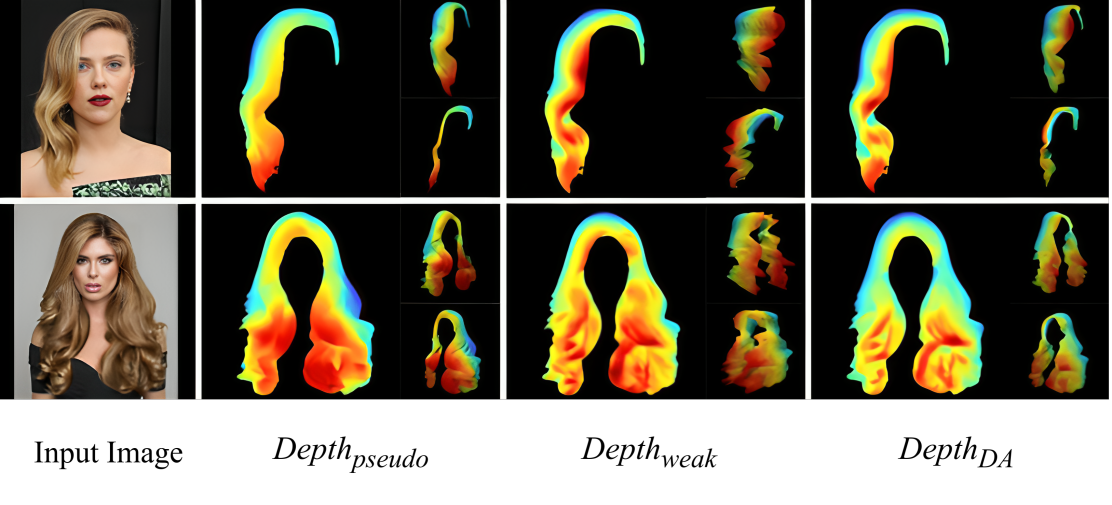
\includegraphics[width=0.9\textwidth]{assets/figures/eval/hairrida/depth-comparison.png}
        \caption{Qualitative comparison of predicted depth maps.}
    \end{figure}
\end{frame}

%-----------------------------------------------
% Depth Maps Quantitative Comparison
%-----------------------------------------------
\begin{frame}[t]{Depth Map Estimation: Quantitative Results}
    \textbf{Methods:}
    \begin{itemize}
        \item $Depth_{\text{pseudo}}$: Synthetic pseudo-label-based depth estimation.
        \item $Depth_{\text{weak}}$: Weakly supervised depth estimation using ordinal cues.
        \item $Depth_{\text{DA}}$: Domain-adaptive depth estimation.
    \end{itemize}

    \vspace{5pt}

    \begin{table}[h]
        \renewcommand{\arraystretch}{1.4}
        \centering
        \small
        \begin{tabularx}{0.75\textwidth}{
            >{\raggedright\arraybackslash}X
            >{\centering\arraybackslash}p{3.5cm}
            >{\centering\arraybackslash}p{3.5cm}
        }
            \hline
            \rowcolor{myLightBlue}
            \textbf{Method} & \emph{HairRida} $\uparrow$ & $L_1$ $\downarrow$ \\ \hline
            $Depth_{\text{pseudo}}$ & 80.47\% & - \\ \hline
            $Depth_{\text{weak}}$ & 85.17\% & 0.2470/3.125 \\ \hline
            $Depth_{\text{DA}}$ & \textbf{85.20\%} & \textbf{0.1768/0.1188} \\ \hline
        \end{tabularx}
        \caption{Relative depth accuracy (\emph{HairRida}) and $L_1$ loss comparisons for different depth estimation strategies.}
    \end{table}
\end{frame}

\subsection{Single-View 3D Hair Modeling Comparison}

%-----------------------------------------------
% Single-View 3D Hair Modeling
%-----------------------------------------------
\begin{frame}[t]{Single-View 3D Hair Modeling Comparison}
    \textbf{Methods Compared:}
    \begin{itemize}
        \item HairNet~\cite{Zhou2018SingleViewHR}
        \item DynamicHair~\cite{Yang2019DynamicHM}
        \item NeuralHDHair~\cite{wu2022neuralhdhair}
        \item \textbf{NeuralHDHair* + \emph{HairStep}}: Proposed method.
    \end{itemize}

    \vspace{5pt}
    \textbf{Modifications for NeuralHDHair*:}
    \begin{itemize}
        \item \emph{No luminance map}: Reduces domain gap from varying lighting conditions.
        \item \emph{Omit GrowingNet}: Focus on reconstruction quality, not scalability.
    \end{itemize}
\end{frame}

\begin{frame}{Single-View 3D Hair Modeling: Qualitative Comparison}
    \begin{figure}
        \centering
        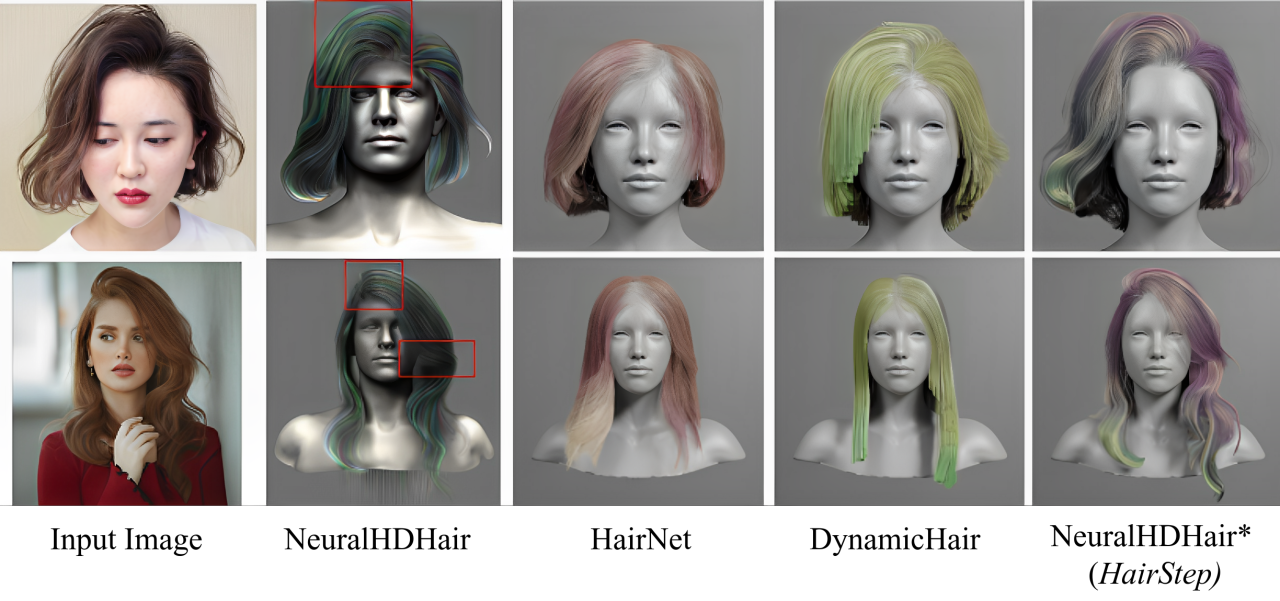
\includegraphics[width=0.7\textwidth]{assets/figures/eval/existing-methods-vis-comparison-1.png}
        \caption{Qualitative comparison with existing single-view 3D hair reconstruction methods.}
    \end{figure}
\end{frame}

\begin{frame}{Single-View 3D Hair Modeling: Additional Comparisons}
    \begin{figure}
        \centering
        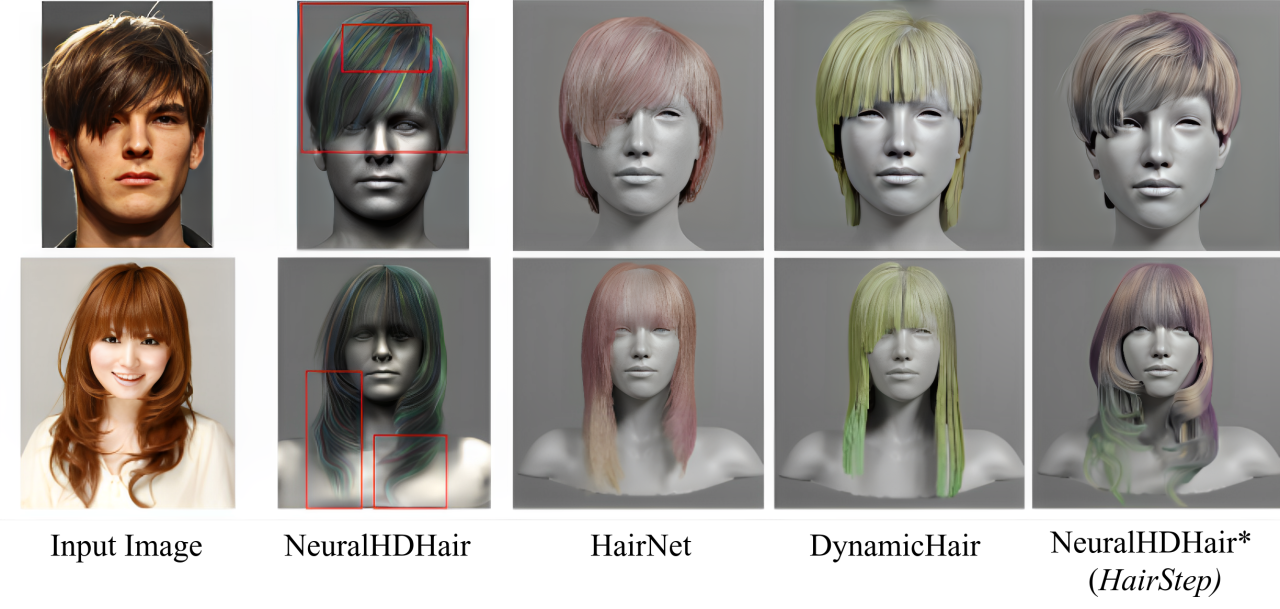
\includegraphics[width=0.7\textwidth]{assets/figures/eval/existing-methods-vis-comparison-2.png}
        \caption{Additional qualitative comparisons with baseline methods.}
    \end{figure}
\end{frame}

\begin{frame}[t]{Single-View 3D Hair Modeling: Observations}
    \textbf{Key Observations:}
    \begin{itemize}
        \item \textbf{HairNet} and \textbf{DynamicHair}:
        \begin{itemize}
            \item Produce coarse, less detailed shapes.
            \item Struggle with complex hairstyles.
        \end{itemize}
        \item \textbf{NeuralHDHair}:
        \begin{itemize}
            \item Faces challenges with sharp depth variations.
            \item Struggles with intricate hair growth patterns.
        \end{itemize}
        \item \textbf{Orientation-based methods}:
        \begin{itemize}
            \item Lack fine-grained detail necessary for accurate 3D reconstruction.
        \end{itemize}
    \end{itemize}
\end{frame}

\subsection{Intermediate Representation Evaluation}

%-----------------------------------------------
% Intermediate Representation Evaluation
%-----------------------------------------------
\begin{frame}[t]{Intermediate Representation Evaluation}
    \textbf{Goal:} Examine how different intermediate representations affect the final 3D hair reconstruction quality.

    \vspace{5pt}
    \textbf{Intermediate Representations:}
    \begin{itemize}
        \item Orientation Map
        \item Strand Map
        \item \emph{HairStep} (Strand + Depth Maps)
    \end{itemize}

    \textbf{Methods:}
    \begin{itemize}
        \item HairNet~\cite{Zhou2018SingleViewHR}
        \item DynamicHair~\cite{Yang2019DynamicHM}
        \item NeuralHDHair* + \emph{HairStep}
    \end{itemize}
\end{frame}

%-----------------------------------------------
% Intermediate Representation -- Synthetic Data
%-----------------------------------------------
\begin{frame}[t]{Quantitative Results on Synthetic Data}
    \begin{table}[h]
        \centering
        \small
        \renewcommand{\arraystretch}{1.4}
        \begin{tabular}{l|c|c}
            \hline
            \rowcolor{myLightBlue}
            Method & Orientation Error $\downarrow$ & Occupancy Accuracy $\uparrow$ \\
            \hline
            HairNet (Orientation Map) & 0.02349 & -- \\
            HairNet (Strand Map) & 0.02206 \textcolor{blue}{(-6.1\%)} & -- \\
            HairNet (HairStep) & \textbf{0.02184} \textcolor{blue}{(-7.0\%)} & -- \\
            \hline
            DynamicHair (Orientation Map) & 0.1352 & 78.19\% \\
            DynamicHair (Strand Map) & 0.1185 \textcolor{blue}{(-12.4\%)} & 79.62\% \\
            DynamicHair (HairStep) & \textbf{0.1174} \textcolor{blue}{(-13.2\%)} & \textbf{79.78\%} \\
            \hline
            NeuralHDHair* (Orientation Map) & 0.1324 & 82.59\% \\
            NeuralHDHair* (Strand Map) & 0.0722 \textcolor{blue}{(-41.7\%)} & 84.18\% \\
            NeuralHDHair* (HairStep) & \textbf{0.0658} \textcolor{blue}{(-50.3\%)} & \textbf{86.77\%} \\
            \hline
        \end{tabular}
        \caption{Quantitative results on synthetic data (USC-HairSalon). \emph{HairStep} consistently improves performance.}
        \label{tab:representation_effectiveness_synthetic}
    \end{table}
\end{frame}

%-----------------------------------------------
% Intermediate Representation -- Real Data
%-----------------------------------------------
\begin{frame}[t]{Quantitative Results on Real Data}
    \begin{table}[h]
        \centering
        \small
        \renewcommand{\arraystretch}{1.4}
        \begin{tabular}{l|c|c|c}
            \hline
            \rowcolor{myLightBlue}
            Method & IoU $\uparrow$ & \emph{HairSale} $\downarrow$ & \emph{HairRida} $\uparrow$ \\
            \hline
            HairNet (Orientation Map) & 57.15\% & 31.97 & 75.65\% \\
            HairNet (Strand Map) & 57.48\% & 28.60 \textcolor{blue}{(-10.5\%)} & 74.81\% \\
            HairNet (HairStep) & 57.01\% & \textbf{27.68} \textcolor{blue}{(-13.4\%)} & \textbf{74.97\%} \\
            \hline
            DynamicHair (Orientation Map) & 56.39\% & 32.66 & 74.08\% \\
            DynamicHair (Strand Map) & 59.51\% & \textbf{26.53} \textcolor{blue}{(-18.8\%)} & 73.42\% \\
            DynamicHair (HairStep) & 59.14\% & 27.51 \textcolor{blue}{(-15.8\%)} & \textbf{73.58\%} \\
            \hline
            NeuralHDHair* (Orientation Map) & 77.56\% & 19.60 & 70.67\% \\
            NeuralHDHair* (Strand Map) & 77.60\% & \textbf{16.00} \textcolor{blue}{(-18.4\%)} & 72.37\% \\
            NeuralHDHair* (HairStep) & 77.22\% & 16.36 \textcolor{blue}{(-16.5\%)} & \textbf{76.79\%} \\
            \hline
        \end{tabular}
        \caption{Quantitative comparisons on real data. \emph{HairStep} yields consistently improved performance.}
        \label{tab:representation_effectiveness_real}
    \end{table}
\end{frame}

%-----------------------------------------------
% Intermediate Representation -- Real Data Qualitative
%-----------------------------------------------
\begin{frame}{Qualitative Comparison on Real Data}
    \begin{figure}
        \centering
        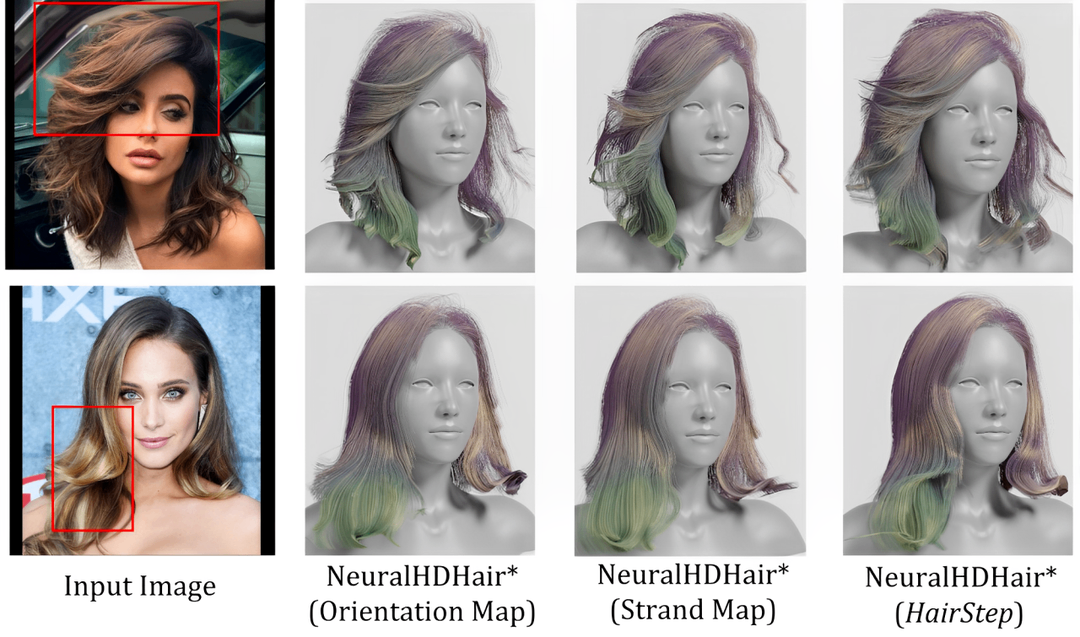
\includegraphics[width=0.6\textwidth]{assets/figures/eval/neuralhdhair.png}
        \caption{Qualitative results of NeuralHDHair* using (left to right) orientation map, strand map, and \emph{HairStep}.}
    \end{figure}
\end{frame}

%-----------------------------------------------
% Intermediate Representation Impact Observations
%-----------------------------------------------
\begin{frame}[t]{Intermediate Representation Impact: Observations}
    \emph{HairStep} consistently improves performance on both synthetic and real data.

    \vspace{5pt}
    \textbf{User Study (10 samples, 39 participants):}
    \begin{itemize}
        \item 64.87\% preferred reconstructions using \emph{HairStep}.
        \item 21.28\% preferred strand map-based reconstructions.
        \item 13.85\% preferred orientation map-based reconstructions.
    \end{itemize}
\end{frame}

\subsection{Ablation Study}

%-----------------------------------------------
% Ablation Studies
%-----------------------------------------------
\begin{frame}[t]{Ablation Study: Depth Estimation}
    \textbf{Objective:} Evaluate the impact of different depth estimation approaches on final reconstruction.

    \vspace{5pt}
    \textbf{Configurations:}
    \begin{itemize}
        \item $C_0$: Strand Map + $Depth_{\text{pseudo}}$
        \item $C_1$: Strand Map + $Depth_{\text{weak}}$
        \item \textbf{Full}: Strand Map + $Depth_{\text{DA}}$
    \end{itemize}

    \vspace{5pt}
    \begin{table}[h]
        \centering
        \small
        \renewcommand{\arraystretch}{1.4}
        \begin{tabularx}{0.75\textwidth}{
            >{\raggedright\arraybackslash}X
            >{\centering\arraybackslash}X
            >{\centering\arraybackslash}p{2.5cm}
            >{\centering\arraybackslash}p{2.5cm}
        }
            \hline
            \rowcolor{myLightBlue}
            Method & IoU $\uparrow$ & \emph{HairSale} $\downarrow$ & \emph{HairRida} $\uparrow$ \\
            \hline
            $\mathbf{C_0}$ & 77.75\% & 16.03 \textcolor{blue}{(-18.2\%)} & 73.57\% \\
            $\mathbf{C_1}$ & 77.11\% & 16.54 \textcolor{blue}{(-15.6\%)} & 75.80\% \\
            \textbf{Full} & \textbf{77.22\%} & \textbf{16.36} \textcolor{blue}{(-16.5\%)} & \textbf{76.79\%} \\
            \hline
        \end{tabularx}
        \caption{Ablation study: Evaluating depth estimation methods within the \emph{HairStep} framework.}
    \end{table}
\end{frame}

%-----------------------------------------------
% Ablation Studies Visualization
%-----------------------------------------------
\begin{frame}{Ablation Study: Configurations Comparison}
    \begin{figure}
        \centering
        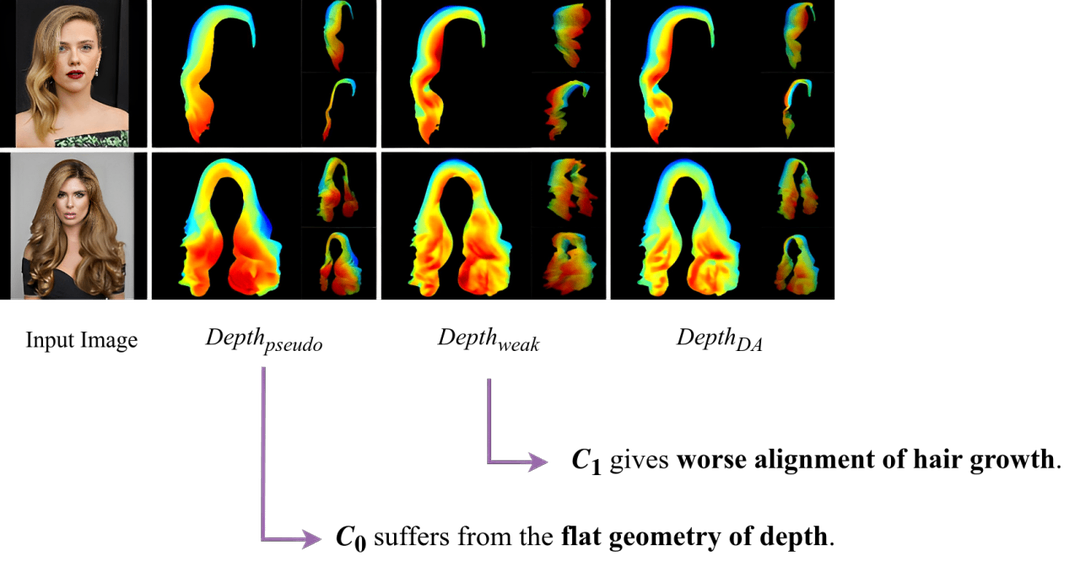
\includegraphics[width=0.8\textwidth]{assets/figures/eval/ablation/depth-comparison.png}
        \caption{Qualitative comparison of different depth estimation configurations.}
    \end{figure}
\end{frame}

%-----------------------------------------------
% Ablation Studies Qualitative Example
%-----------------------------------------------
\begin{frame}{Ablation Study: Visual Comparison}
    \begin{figure}
        \centering
        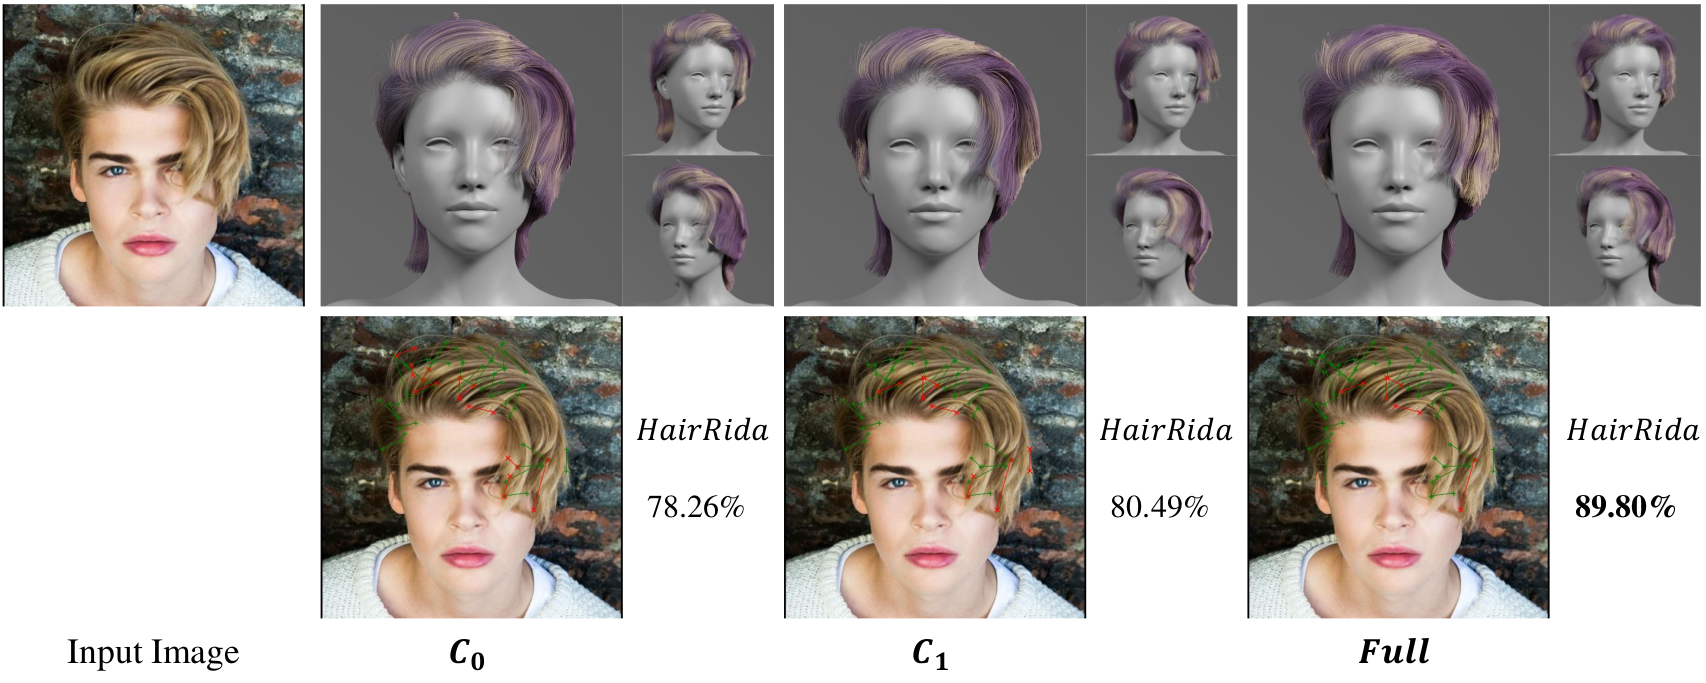
\includegraphics[width=0.8\textwidth]{assets/figures/eval/ablation/sample-1.png}
        \caption{From left to right: Input image, $C_0$, $C_1$, and Full method. Green/red lines indicate correct/incorrect relative depth predictions (\emph{HairRida}).}
    \end{figure}
\end{frame}
